% HMC Math dept HW template example
% v0.04 by Eric J. Malm, 10 Mar 2005
\documentclass[12pt,letterpaper,boxed,cm]{hmcpset}

% set 1-inch margins in the document
\usepackage[margin=1in]{geometry}
\usepackage{mathtools}
\usepackage{mathrsfs}
% include this if you want to import graphics files with /includegraphics
\usepackage{graphicx}
\usepackage{cases}
\usepackage{hyperref}
\usepackage{siunitx}
\usepackage{tikz}
\usepackage{cases}
\usepackage{mathalfa}
\usetikzlibrary{arrows}

% info for header block in upper right hand corner
\name{Name: ~~~~~~~~~~~~~~~~~~~~~~~~~~~~~~~}
\class{Physics 51}
\assignment{Homework \#17}
\duedate{November 7, 2016}

\newcommand{\ev}[2]{\Big|_{#1}^{#2}}
\newcommand{\evv}[2]{\Big|_{#1}^{#2}}
\newcommand{\set}[1]{\left\{#1\right\}}
\newcommand{\s}[1]{\sqrt{#1}}
\newcommand{\f}[2]{\frac{#1}{#2}}
\newcommand{\p}[2]{\frac{\partial #1}{\partial #2}}
\providecommand{\t}[1]{\text{#1}}
\providecommand{\span}[1]{\text{span}\left(#1\right)}
\providecommand{\set}[1]{\left\{#1\right\}}
\providecommand{\l}[0]{\left}
\providecommand{\r}[0]{\right}
\newcommand{\m}[1]{\begin{matrix}#1\end{matrix}}
\newcommand{\bm}[1]{\begin{bmatrix}#1\end{bmatrix}}
\renewcommand{\bf}[1]{\mathbf{#1}}
\newcommand{\pn}[1]{\left( #1 \right)}
\newcommand{\abs}[1]{\left| #1 \right|}
\newcommand{\bk}[1]{\left[ #1 \right]}
\newcommand{\cis}[1]{\pn{\cos\pn{#1} + i\sin\pn{#1}}}
\newcommand{\cisi}[1]{\pn{\cos\pn{#1} - i\sin\pn{#1}}}
\renewcommand{\Im}[1]{\text{Im}\pn{#1}}
\renewcommand{\Re}[1]{\text{Re}\pn{#1}}
\renewcommand{\k}[0]{\f{1}{4\pi\epsilon_0}}
\renewcommand{\part}[1]{\vspace{1em}\noindent(#1)}

\makeatletter
\renewcommand*\env@matrix[1][*\c@MaxMatrixCols c]{%
  \hskip -\arraycolsep
  \let\@ifnextchar\new@ifnextchar
  \array{#1}}
\makeatother
\begin{document}
\problemlist{38-E25, 38-E28, 38-P13*, 38-P14}

\begin{problem}[38-E25]
The intensity of direct solar radiation not absorbed by the atmosphere on a particular summer day is \SI{130}{W/m^2}. How close would you have to stand to a $1.0$-$\SI{}{kW}$ electric heater to feel the same intensity? Assume that the heater radiates uniformly in all directions.
\end{problem}
\begin{solution}
\end{solution}
\newpage

\begin{problem}[38-E28]
Sunlight strikes the Earth, just outside its atmosphere, with an intensity of \SI{1.38}{kW/m^2}. Calculate
\begin{enumerate}
	\item[(a)] $E_m$ and 
	\item[(b)] $B_m$ for sunlight, 
\end{enumerate}
assuming it to be plane wave.
\end{problem}
\begin{solution}
\end{solution}
\newpage

\begin{problem}[38-P13*]
A plane electromagnetic wave, with wavelength \SI{3.18}{m}, travels in free space in the $+x$ direction with its electric field vector $\vec{\mathbf{E}}$, of amplitude \SI{288}{V/m}, directed along the $y$ axis.
\begin{enumerate}
	\item[(a)] What is the frequency of the wave?
	\item[(b)] What is the direction and amplitude of the magnetic field associated with the wave?
	\item[(c)] If $E = E_m\sin\pn{kx-\omega t}$, what are the values of $k$ and $\omega$?
	\item[(d)] Find the intensity of the wave.
	\item[(e)] If the wave falls on a perfectly absorbing sheet of area \SI{1.85}{m^2}, at what rate would momentum be delivered to the sheet and what is the radiation pressure exerted on the sheet?
\end{enumerate}
\end{problem}
\begin{solution}
\end{solution}
\newpage

\begin{problem}[38-P14]
Figure 38-30 shows a parallel-plate capacitor being charged.

\begin{enumerate}
	\item[(a)] Show that the Poynting vector $\vec{S}$ points everywhere radially into the cylindrical volume.
	\item[(b)] Show that the rate at which energy flows into this volume, calculated by integrating the Poynting vector over the cylindrical boundary of this volume, is equal to the rate at which the stored electrostatic energy increases; that is,
	\[
		\int \vec{S} \cdot d\vec{A} = Ad\f{d}{dt}\pn{\f{1}{2}\epsilon_0E^2},
	\]
	where $Ad$ is the volume of the capacitor and $\f{1}{2}\epsilon_0E^2$ is the energy density for all points within that volume. This analysis shows that, according to the Poynting vector point of view, the energy stored in a capacitor does not enter it through the wires but through the space around the wires and the plates. (Hint: To find $\vec{S}$ we must first find $\vec{B}$, which is the magnetic field set up by the displacement current during the charging process; see Fig. 38-2. Ignore fringing of the lines of $\vec{E}$.
\end{enumerate}
\begin{center}
	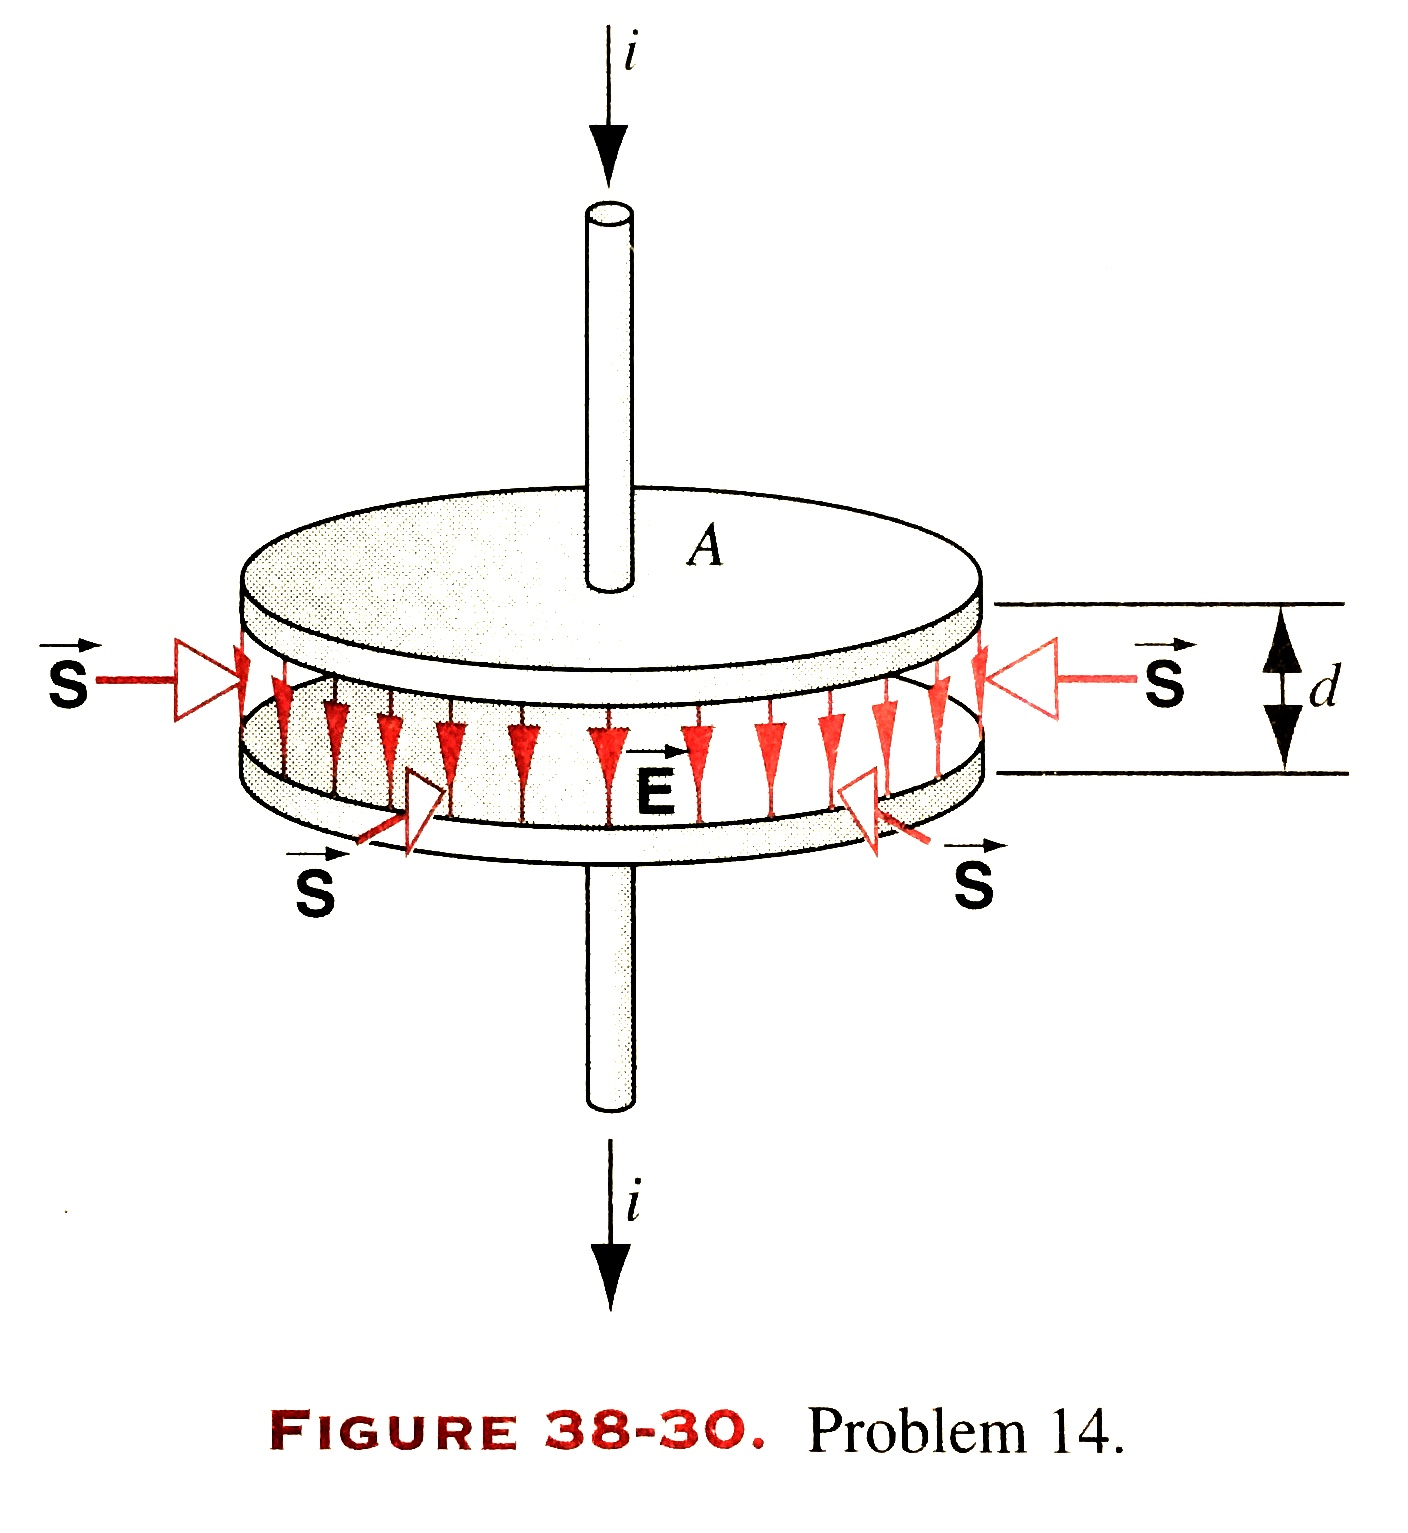
\includegraphics[scale=0.1]{01.jpg}
\end{center}
\end{problem}
\begin{solution}
\end{solution}


\end{document}